\section{Implementation}
\label{section:implementation}
The Destination Choice model described in this thesis was designed as a component of a larger long distance model for the Ministry of Transportation, Ontario. This long distance model is being developed in the JAVA programming language as a traditional 4-step model. 

In the trip generation phase, a list of trips without destinations is generated for a synthetic population of households and persons. These trips are then passed into the destination choice model, which assigns a destination for each trip. For each trip the destination choice model is run, returning a predicted destination for that trip. For the calibration and scenario analysis, the observed dataset was used. The full expanded trip records numbers 362 million trips, and the model implementation currently cannot hold that many trips in memory. Therefore a sample of 1,000,000 trips is made by performing random draws from the observed dataset, based on the trip weight.

The algorithm works as followed, with step~\ref{item:trip} being performed across the list of trips in parallel. 

\begin{enumerate}
\item A Destination Choice Model is initialized with the following:
	\begin{itemize}
	\item Coefficients for each model strata
	\item Destination zones and their attributes
	\item The distance matrix between zones
	\end{itemize}
\item \label{item:trip} For each trip:
	\begin{enumerate}
	\item Calculate the utility $u_j$ for each destination $j$, using the relevant stored coefficients.
	\item \label{item:denom} calculate the denominator of the logit equation $q = {\sum_{j=1}^{J} e^{u_j}}
	$
	\item Calculate the probability of each destination $j$, $P(j) = e^{u_j} / q $
	\item Choose a destination based on the probabilities using an \textit{EnumeratedIntegerDistribution} from the Apache commons math library 
	\begin{verbatim}
	return new EnumeratedIntegerDistribution(alternatives, probabilities).sample();
	\end{verbatim}

	\item store the destination in the trip object
	\end{enumerate}
\end{enumerate}

\section{Calibration}

The implemented model was calibrated for each trip purpose against the observed average trip length. Through trial and error, the coefficient of the exponential distance term was multiplied by a factor $k$ to adjust the predicted trip length. The results of the calibration are presented in table~\ref{table:calibration}. Figure~\ref{fig:overall-calibration} shows the results of the calibration for the overall model, as displayed in a trip length distribution. Then end result is acceptable. The two peaks after 3,000 km, representing connections to British Columbia and Alberta are visible in the predicted trip length distribution. The individual trip length distributions for business, leisure and visit purposes are available in the appendix. 


\begin{table}[H]
\centering
\caption{Calibration coefficients and on average trip length}
\label{table:calibration}
\begin{tabular}{@{}rrrrrr@{}}
  \toprule
 &  & \multicolumn{3}{c}{Average trip length (km)} \\ \midrule
 Trip purpose & $k$ & observed & estimated & calibrated & $\Delta$ \\ \midrule
  Business & 1.05 & 377 & 408 & 391 & 3.6\% \\ 
  Leisure & 1.15 & 212 & 264 & 214  & 0.9\% \\
  Visit  & 1.15  & 232 & 213 & 236  & 1.7\%\\   \midrule
  Total  &  & 245 & 318 & 249 & 1.6\% \\ 
   \bottomrule
\end{tabular}
\end{table}

\begin{figure}[H]
\centering
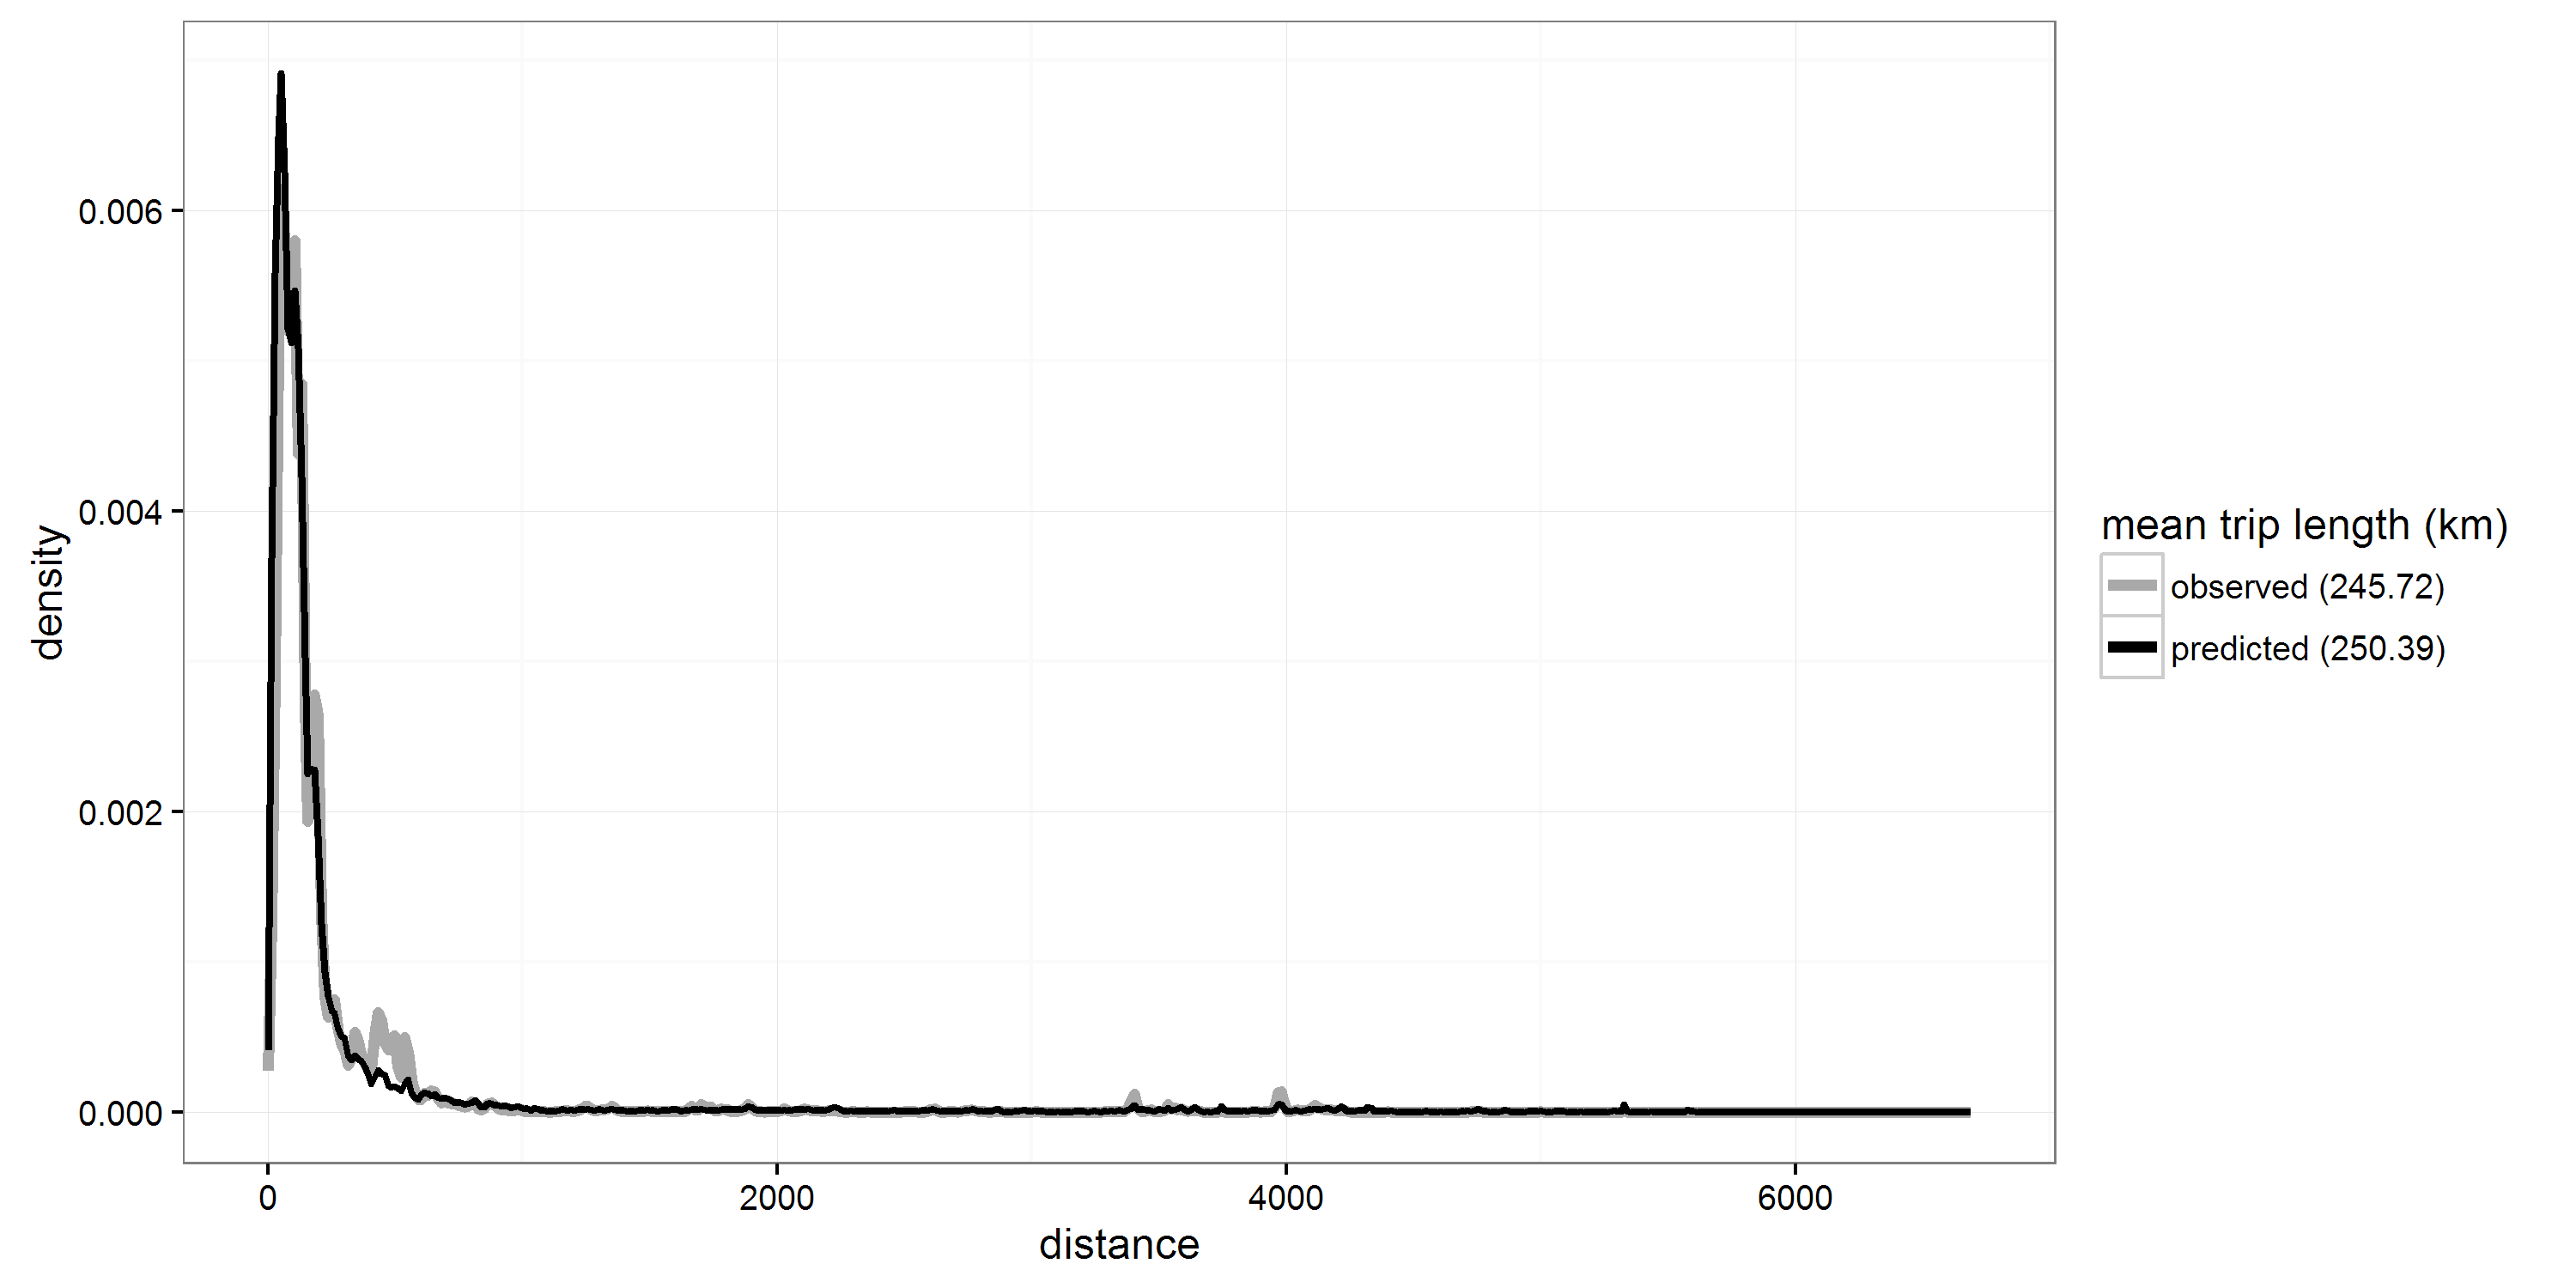
\includegraphics[width=0.8\textwidth]{calibration/m6_calibrated}
\caption{Trip length distribution of model \textit{m6} after calibration}
\label{fig:overall-calibration}
\end{figure}


\section{Scenario analysis - Case study of a new ski resort}
\label{scenario-analysis}

This section presents a hypothetical application of the developed destination choice model. For any large scale land use planning or development, it is important to model the impacts that such development will have on the transport network. As an example of this, a hypothetical scenario of the development of a large new ski resort is presented. Such resorts not only provide infrastructure for skiing and other snow-based activities, but require the development of multiple new hotels, employee housing, and retail infrastructure. In the winter months, ski resorts can generate significant demands on the transport network, and this needs to be taken account when considering such a development.

In the hypothetical scenario, a new resort is proposed for the highlands area north of Toronto  in Dufferin (Toronto CMA) (see figure~\ref{fig:scenario-map}. The higher elevation ensures good snowfall, and the elevation difference makes for exciting riders for snow sports enthusiasts. Two sites are being considered, one to the west of the range, and one to the east, closer to Ottawa. While this resort can naturally not be the size of mega resorts in British Columbia or Alberta, its development is expected to bring similar numbers of visitors as other large resorts in Ontario. Three average sized hotels will also be built at the base of the resort to accommodate guests. In the summer, the resort will attract visitors by providing mountain biking facilities and hiking. Additional housing for 400 new residents will be required to support 300 jobs.

\begin{figure}[H]
\centering
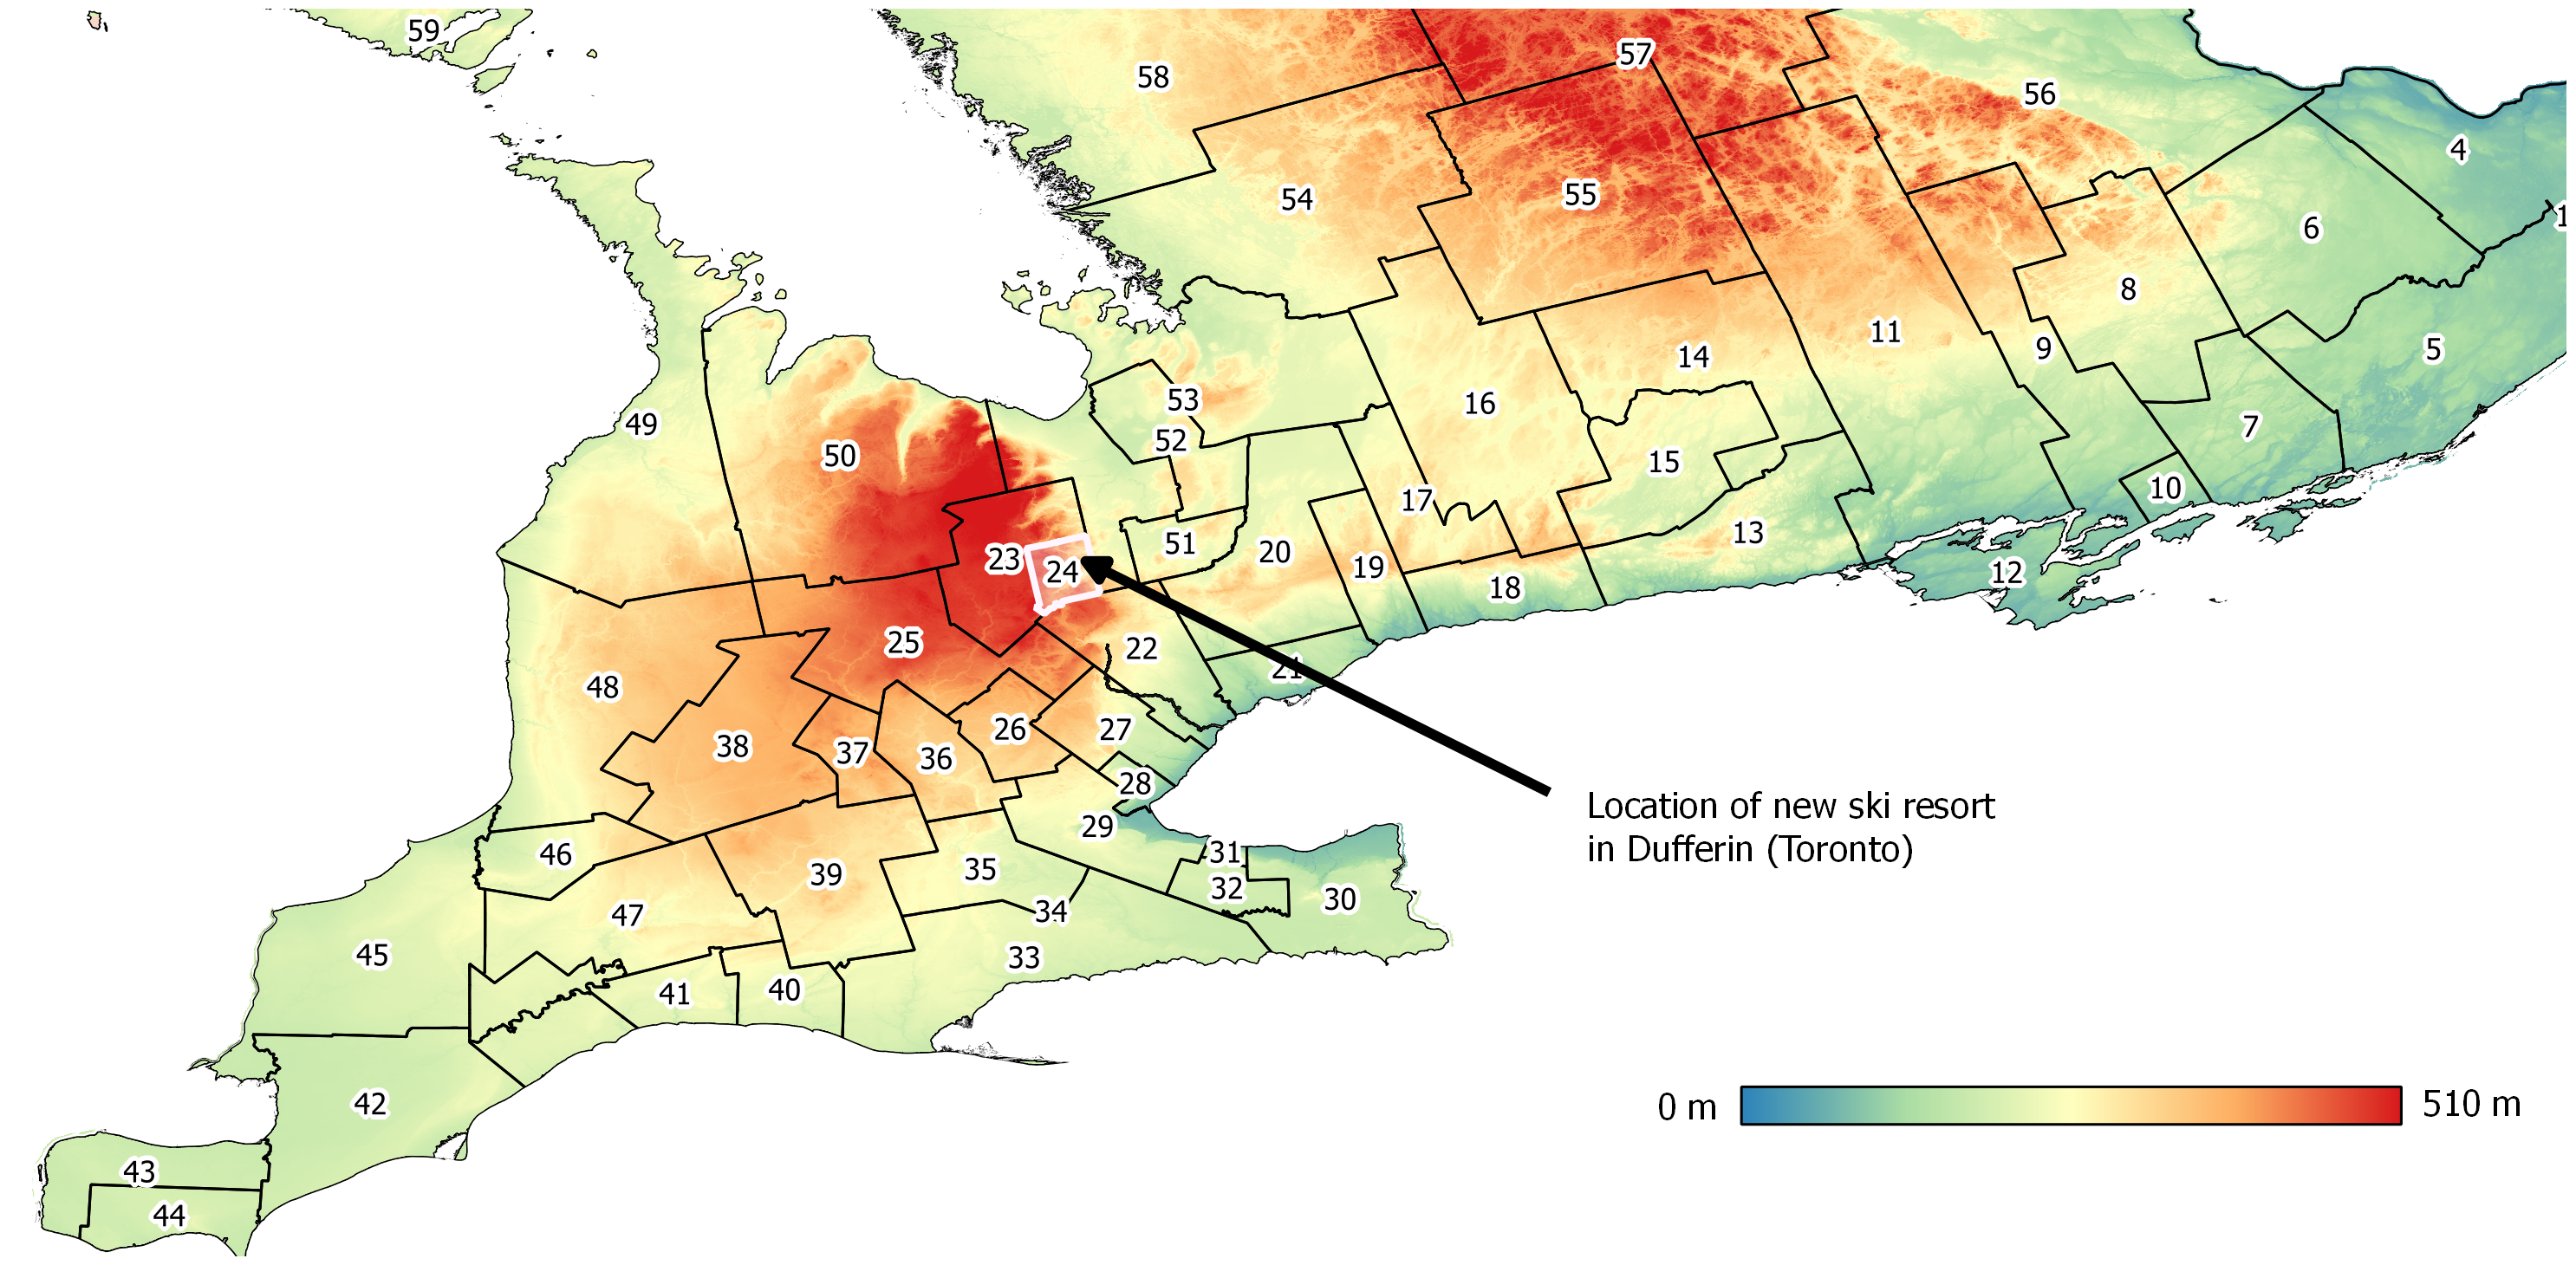
\includegraphics[width=\textwidth]{scenario_map}
\caption{Scenario analysis: Location of a new ski resort on Dufferin (Toronto CMA). Elevation data from the Ontario Provincial Digital Elevation Model - Version 3.0 }
\label{fig:scenario-map}
\end{figure}

This somewhat contrived scenario assumes that other policy and development considerations, such as site location and transport access have all been dealt with. The design of the scenario presents the opportunity to investigate the sensitivity of the  variables based on the foursquare data. The variables concerned are hotels, skiing and outdoor. The impact of the new development is estimated through adjusting these variables for the zone in which the development will take place. The foursquare POI database developed in section~\ref{section:foursquare} was used to estimate adjustments for each of the categories. Taking all venues in Ontario, the average number of checkins per venue for each search category was calculated. The following adjustments are made for the respective zones, and their values are displayed in table~\ref{table:scenario-inputs}.

\begin{minipage}{\textwidth}
\begin{itemize}
\item Skiing: The average number of checkins for ski areas
\item Hotel: Twice the average number of checkins for hotels
\item Outdoor: The average number of checkins per outdoor venue
\end{itemize}
\end{minipage}

%TODO zone 
\begin{table}[H]
\centering
\caption{Inputs for sensitivity analysis scenario}
\label{table:scenario-inputs}
\begin{tabular}{@{}rlll@{}}
  \toprule
 Parameter & Old Value & Adjustment & New Value  \\ \midrule
  $civic_{ij}$ & 42,216 & 700 & 42,916  \\ 
  $hotel_j$ & 1,393  & 8,304 & 9,697  \\ 
  $outdoors_j$  & 1 & 3,389 & 3,390  \\ 
  $skiing_j$ & 40  & 3,550 & 3,590 \\ 
   \bottomrule
\end{tabular}
\end{table}

The trips from the TSRC data used for estimation were inputted to the scenario, with $n/(365*4)$ copies of each record added to the trip table, where $n$ is the trip weight of the record. The weighted TSRC data represents the total trips over 4 years, and for simplicity, the weights are scaled to give the approximate number of daily trips. 20 iterations of the scenario were performed to account for the stochastic nature of destination choice. Figure~\ref{fig:scenario-results} shows the increase in incoming trips to Dufferin due to the new ski resort. The impacts of each input is presented from left to right, with the most right column being to total impact of the combined parameters. 

\begin{figure}[H]
\centering
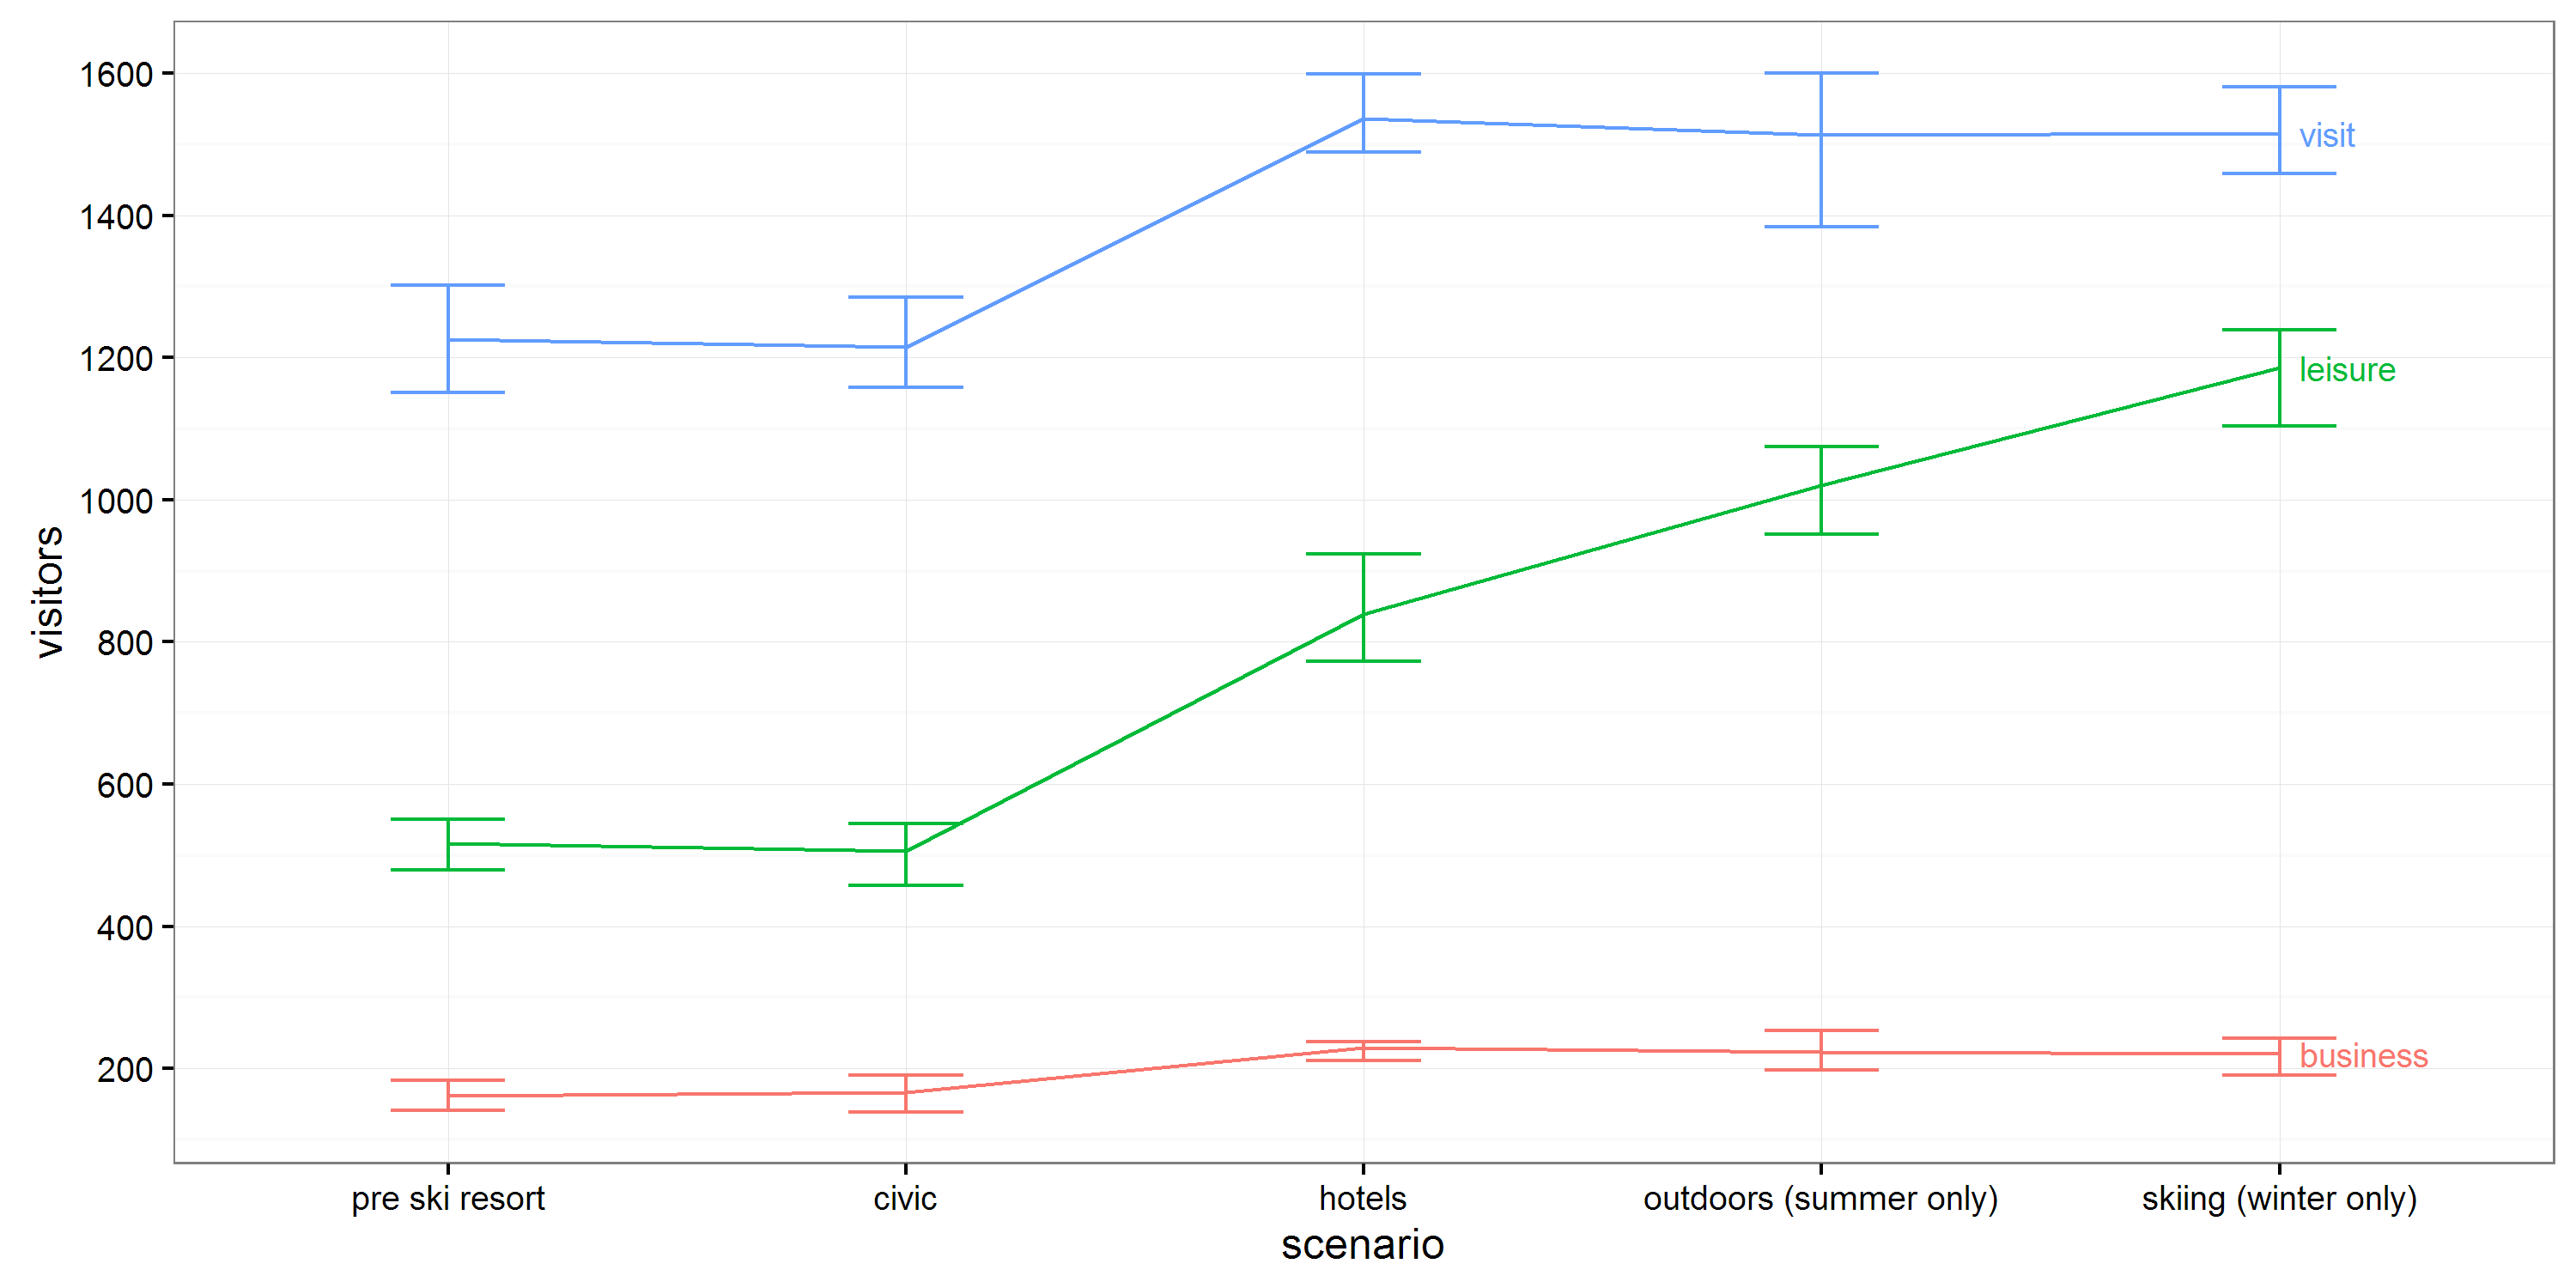
\includegraphics[width=\textwidth]{scenario_analysis}
\caption{Scenario analysis: Impact of a new ski resort on Dufferin (Toronto CMA)}
\label{fig:scenario-results}
\end{figure}


\section{Remaining implementation work}
This thesis presents an operational destination choice model for domestic travel to and from Ontario. The U.S.-Ontario border is an important source of incoming trips to Ontario and external trips that pass through to other parts of Canada. Further work is needed to extend the model to include firstly continental travel to the United States, and then also intercontinental travel. The Canadian International Travel Survey (ITS) provides trip records that can be used to estimate such a model, although it does not include socioeconomic data for travelers. 

%train dest choice log
For a fully functional transport model, the trip ends of the completely specified trips will have to be allocated to the higher resolution TAZs before route assignment can take place. This can be performed before or after mode choice. \textcite{Train09} discusses the issue of geographical aggregation, specifically in regards to destination choice in chapter 3 of \textit{Discrete Choice Methods with Simulation}, 
``to specify a destination choice model that is not sensitive to the level of zonal aggregation, representative utility needs to be specified with parameters inside a log operation."
As all parameters that actually represent destination utility (population and employment, and foursquare categorical variables) have been transformed with a logarithmic function, The model should be insensitive to the resolution of the zone system, and the estimated coefficients transferable to a an choice set of alternatives based on the TAZs of the larger transport model.
